\section{Численный метод}

Перед тем, как перейти к исследованию полной задачи \ref{matrix_equation} в трёхмерной постановке, рассмотрим одномерное уравнение вида
\begin{equation}
\frac{\partial\vec{u}}{\partial{t}}+\mathbf{A}\frac{\partial\vec{u}}{\partial{x}}=0.
\label{advection_equation}
\end{equation}

\subsection{Решение одномерной задачи}

\subsubsection{Гиперболические свойства системы уравнений}
\label{sec:hyperbolic_features}

Если матрица $\mathbf{A}$ имеет полный набор вещественных собственных значений, 
то такое уравнение называется гиперболическим, и его решения соответствуют 
процессам, которые носят волновой характер. Спектральное исследование матриц $\mathbf{A}_x$, $\mathbf{A}_y$, $\mathbf{A}_z$ проведено в \cite{chelnokov}, где показано, что для них существует полный набор собственных значений и собственных векторов.

В этом случае для любой из матриц $\mathbf{A}_x$, $\mathbf{A}_y$, $\mathbf{A}_z$ существует разложение:
\begin{equation}
\mathbf{A}=\mathbf\Omega^{-1}\mathbf\Lambda\mathbf\Omega,
\end{equation}
где $\mathbf\Omega$ -- матрица, строки которой $\vec\omega_i^T$ являются собственными для матрицы $\mathbf A$ и
удовлетворяют соотношениям
\begin{equation}
\vec\omega_i^T\mathbf A=\lambda_i\vec\omega_i^T
\end{equation}
или, что то же самое, транспонированные строки $\mathbf\Omega$ являются собственными векторами для матрицы $\mathbf A^T$
\begin{equation}
\mathbf A^T\vec\omega_i=\lambda_i\vec\omega_i.
\end{equation}
Здесь $\mathbf\Lambda=diag\{\lambda_i\}$ -- диагональная матрица соответствующих собственных значений.

Домножив уравнение \ref{advection_equation} слева на $\mathbf\Omega$, получаем уравнение
\begin{equation}
\frac{\partial{\mathbf\Omega{\vec u}}}{\partial t}+
\Lambda\frac{\partial{\mathbf\Omega{\vec u}}}{\partial x}=0,
\end{equation}
которое после перехода к инвариантам Римана ${\vec v}=\mathbf\Omega{\vec u}$ приобретает вид
\begin{equation}
\frac{\partial{\vec v}}{\partial t}+
\Lambda\frac{\partial{\vec v}}{\partial x}=0
\end{equation}
и тем самым распадается на $n$ одномерных уравнений вида
\begin{equation}
\frac{\partial{v_i}}{\partial t}+\lambda_i\frac{\partial{v_i}}{\partial x}=0.
\label{advection_equation_splitted}
\end{equation}
Таким образом, решение уравнения \ref{advection_equation} представляется в виде
суммы плоских волн, движущихся со скоростями $\lambda_i$.


\subsubsection{Сеточно-характеристический метод}
\label{sec:gcm_method_idea}

После перехода к инвариантам Римана получено 9 независимых уравнений переноса вида \ref{advection_equation_splitted}. Рассмотрим уравнение такого вида подробнее. Вдоль характеристических кривых $\Gamma$, таких что
\begin{equation}
\label{characteristics}
\frac{dx}{dt} = \lambda,
\end{equation}
уравнение \ref{advection_equation_splitted} принимает вид 
\begin{equation}
\label{characteristic_equation}
\frac{dv_i}{dt} = 0.
\end{equation}
Таким образом, значения инвариантов Римана переносятся с временного слоя $n$ на временной слой $n+1$ вдоль характеристических кривых $\Gamma$. При этом очевидно, что значения $\lambda_i$ будут разные в зависимости от вида матрицы $\mathbf A$, который определяется используемыми реологическими соотношениями.

\begin{figure}[h]
\center{\includegraphics[width=0.5\textwidth]{eps/gcm-idea.eps}}
\caption{Принципиальная схема сеточно-характеристического метода.}
\end{figure}

Алгоритм поиска значений исходных переменных $\vec u$ в некоторой точке $x_m^{n+1}$ на новом временном слое состоит в следующем. Сначала для матрицы $\mathbf A$ необходимо найти собственные числа $\lambda_i$, которые определяют наклон характеристик \ref{characteristics}, выпущенных из точки $x_m^{n+1}$. После этого для каждой характеристики $\Gamma_i$ можно определить точку $x_{i*}^n$ пересечения с временным слоем $n$.

В точке $x_{i*}^n$ тем или иным способом определяются значения переменных $\vec u_{i*}^n$. Способы реконструкции могут быть различными, в данной работе используется интерполяция по сеточному шаблону на предыдущем временном слое (подробнее см.ниже). По найденным значениям $\vec u_{i*}^n$ вычисляется $i$-ый инвариант Римана $v_{i*}^n$ в точке $x_{i*}^n$. Значение инварианта вдоль $\Gamma_i$ будет перенесено в точку $x_m^{n+1}$ на новом временном слое:
\begin{equation}
v_{im}^{n+1} = v_{i*}^n.
\end{equation}

После того, как в точке $x_m^{n+1}$ описанным образом найдены все 9 инвариантов Римана, можно найти в ней исходные переменные $\vec u$. Так как по определению ${\vec v}=\mathbf\Omega{\vec u}$, то
\begin{equation}
{\vec u}_m^{n+1}=\mathbf\Omega^{-1}{\vec v}_*^n,
\end{equation}
где ${\vec v}_*^n$ -- вектор, составленный из значений $v_{i*}^n$, подсчитанных в соответствующих точках на временном слое $n$. Как описано выше, точки, из которых берутся разные компоненты этого вектора, различны.


\subsubsection{Разностные схемы для структурированных сеток}

При использовании структурированных прямоугольных сеток описанный выше алгоритм для уравнения \ref{advection_equation} после выполнения математических преобразований приводит к известным разностным схемам.

\paragraph{Схема Куранта-Изаксона-Рис.} Данная схема строится на трёхточечном сеточном шаблоне $(m-1, m, m+1)$ и позволяет явно выразить значение $u_m^{n+1}$ на новом временном слое:

\begin{equation}
	\label{CIR scheme}
	u^{n+1}_m = u^n_m - \frac{\tau}{h} \Omega^{-1} \Lambda^+ \Omega (u^n_{m+1} - u^n_m) 
	- \frac{\tau}{h} \Omega^{-1} \Lambda^- \Omega (u^n_m – u^n_{m-1}) .
\end{equation}

Схема обладает первым порядком аппроксимации по времени и пространству $O(h, \tau)$, является монотонной и обеспечивает минимальное размытие волнового фронта среди всех схем первого порядка.

\paragraph{Схема Лакса-Вендрофа.} Данная схема является единственной схемой второго порядка точности на шаблоне $(m-1, m, m+1)$. Схема записывается в виде:

\begin{equation}
	\label{LW scheme}
	u^{n+1}_m = u^n_m - \frac{\tau}{2h} A (u^n_{m+1} - u^n_{m-1})
	 - \frac{\tau^2}{2h^2} A^2 (u^n_{m+1} - 2u^n_m + u^n_{m-1}) .
\end{equation}

Так как схема имеет второй порядок аппроксимации, она обеспечивает более точное воспроизведение формы волнового фронта по сравнению со схемами первого порядка. Однако, она не является монотонной, что приводит к появлению нефизичных численных осцилляций на разрывах точного решения.


\paragraph{Гибридная схема.} Для сочетания достоинств и преодоления недостатков обоих схем используется гибридная схема, являющаяся их линейной комбинацией. Гибридная схема имеет следующий общий вид:

\begin{align}
\label{hybrid scheme}
u^{n+1}_m &= u^n_m - \frac{\tau}{2h} A (u^n_{m+1} - u^n_{m-1}) + \nonumber\\
	 &+ \frac{1}{2} ((1-a) \frac{\tau}{h} \Omega^{-1} |\Lambda| \Omega + a \frac{\tau^2}{h^2} A^2 ) (u^n_{m+1} - 2u^n_m + u^n_{m-1}).
\end{align}

При $a = 0$ схема переходит в схему Куранта-Изаксона-Рис и имеет первый порядок аппроксимации. При $a = 1$ схема переходит в схему Лакса-Вендрофа и имеет второй порядок аппроксимации. Если параметр $a$ выбирается фиксированно из диапазона $0 < a < 1$, то схема называется гибридизованной, а полученной численное решение является некоторым усреднением решений первого и второго порядка. Схема называется гибридной, если значение $a$ выбирается независимо в каждой точке сетки на каждом временном шаге в зависимости от локальных свойств численного решения.

В данной работе использовался критерий переключения опорных схем, предложенный Р.П. Федоренко и основанный на локальной гладкости решения:

\begin{equation}
	\label{Fedorenko criterium}
	\frac{(u^n_{m+1} - 2u^n_m + u^n_{m-1})}{2} \le K \frac{(u^n_{m+1} – u^n_{m-1})}{2} .
\end{equation}

Параметр переключения $K$ подбирается в зависимости от задачи. В данной работе использовалось значение $K = 0.5$. Если условие \ref{Fedorenko criterium} не выполнено, решение считается разрывным и параметр $a$ принимает в данной точке значение $0$. Если условие \ref{Fedorenko criterium} выполнено -- параметр принимает значение $1$.

В результате применения такого подхода гладкие участки решения считаются схемой второго порядка, а разрывные -- схемой первого порядка. Гибридная схема позволяет получить минимальное размытие точного решения, но при этом избежать нефизичных осцилляций на разрывных решениях. На рис. \ref{pic:hybrid-scheme-testing} приведение сравнение схемы первого порядка, второго порядка, гибридной схемы и точного решения. Приведено решение задачи о распространении прямоугольного импульса нагрузки в однородной среде. Ширина импульса составляет 40 узлов сетки, к моменту, изображённому на рисунке, импульс прошел 200 узлов сетки от первоначального положения.

\begin{figure}[h]
\centerline{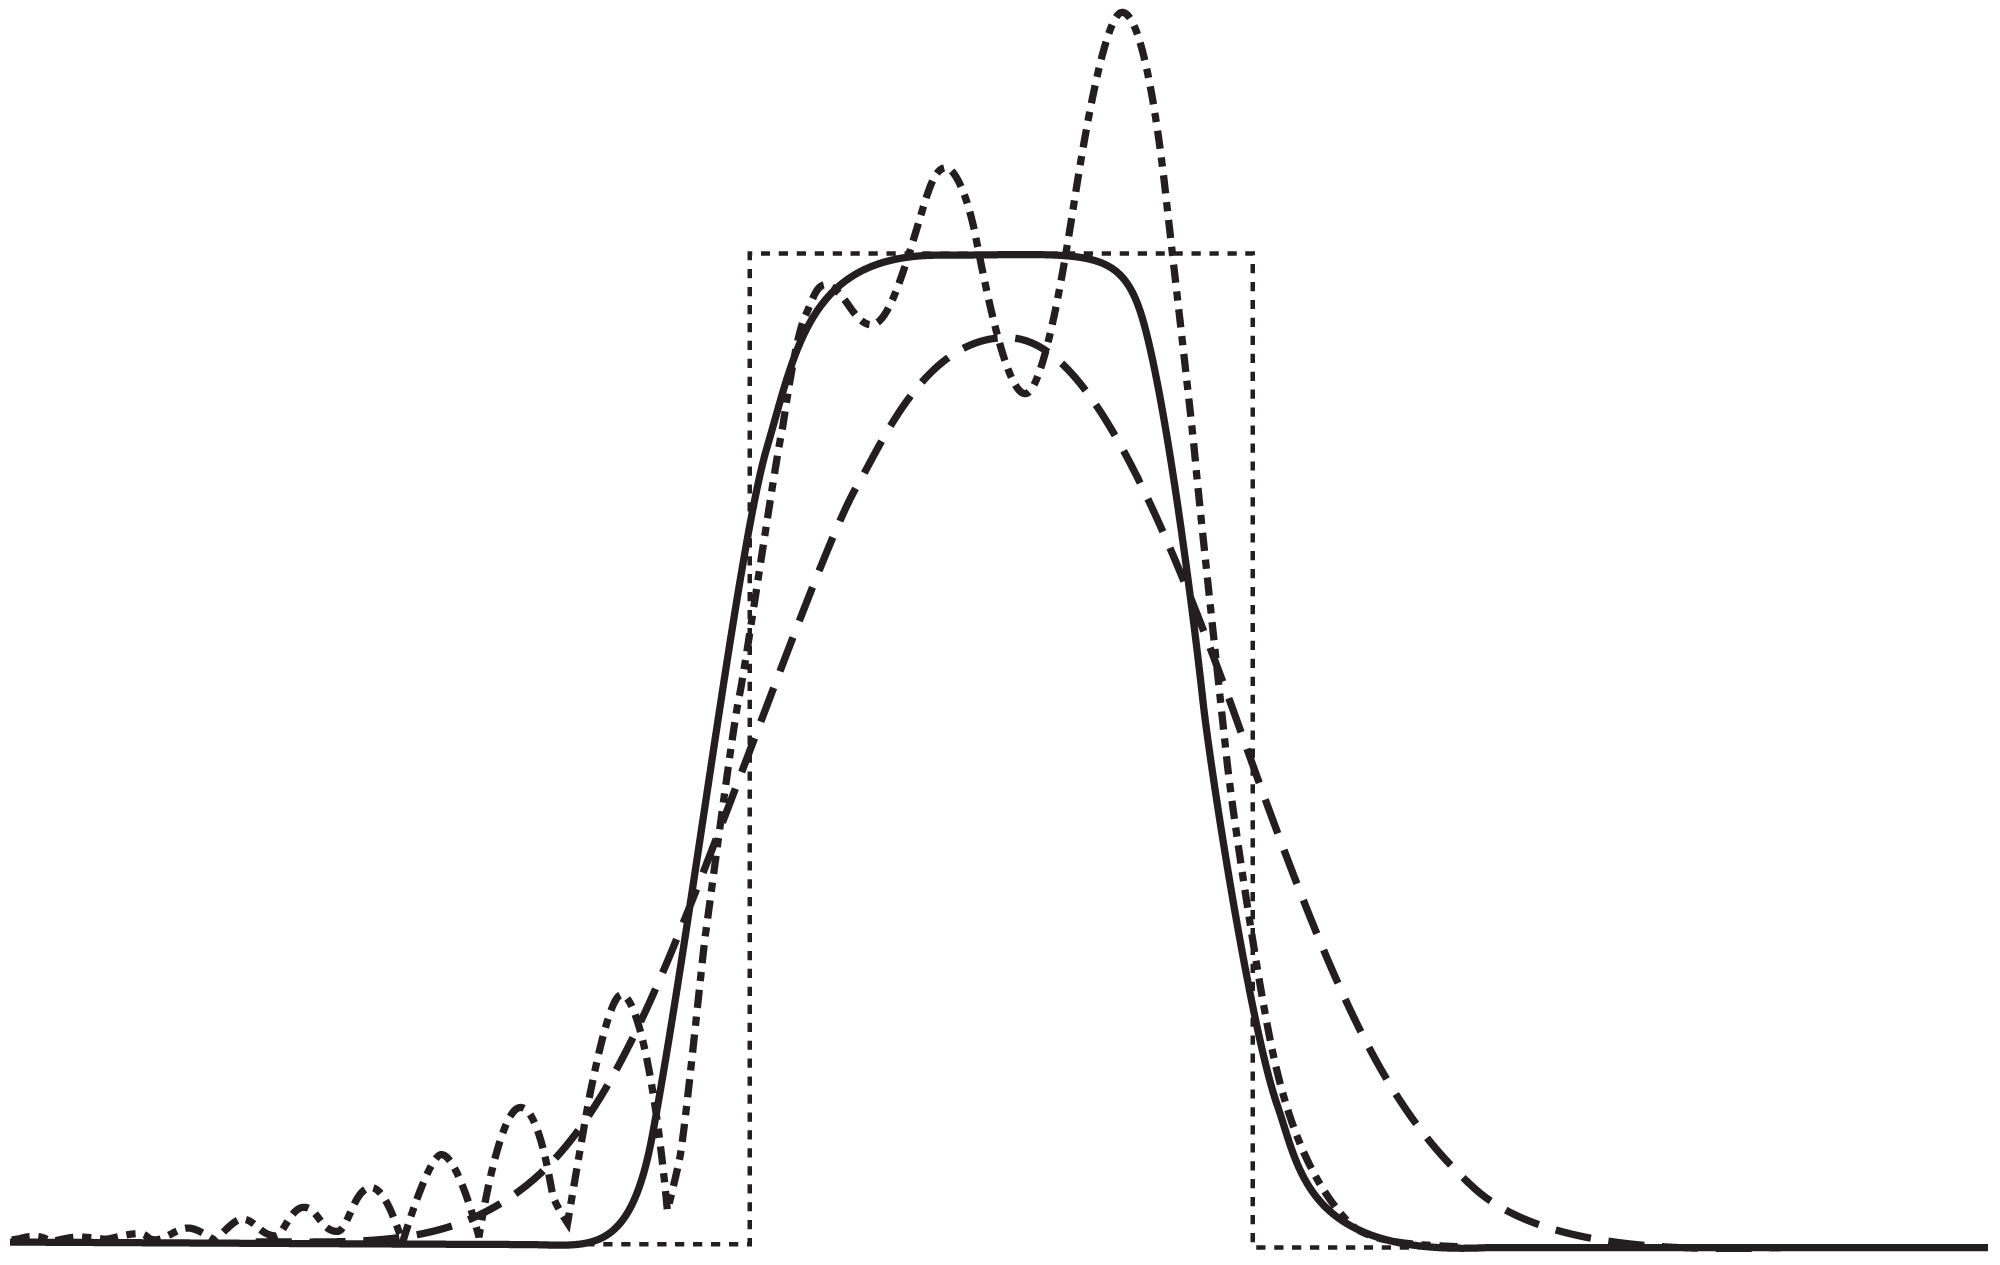
\includegraphics[width=0.75\textwidth]{png/hybrid-scheme-testing.png}}
\caption{Распространение прямоугольного импульса. Штриховая линия -- решение по схеме Куранта-Изаксона-Рис. Штрих-пунктирная -- решение по схеме Лакса-Вендрофа. Сплошная линия -- решение с использованием гибридной схемы. Точками показано точное решение.}
\label{pic:hybrid-scheme-testing}
\end{figure}

\subsubsection{Метод на неструктурированных сетках}

Идея сеточно-характеристического метода на неструктурированных сетках также основана на переносе инвариантов Римана вдоль направления характеристик. В ходе расчёта для каждой характеристики, выпущенной из точки на новом временном слое, по углу наклона $\lambda$ и шагу по времени $\tau$ определяется ячейка сетки на старом временном слое, в который попала данная характеристика (рис. \ref{pic:gcm_2d}). Простейшей формой ячейки неструктурированной сетки для двумерной постановки является треугольник, а для трёхмерной -- тетраэдр. В дальнейшем изложении будем ориентироваться на сетки из тетраэдров.

\begin{figure}[h]
\centering
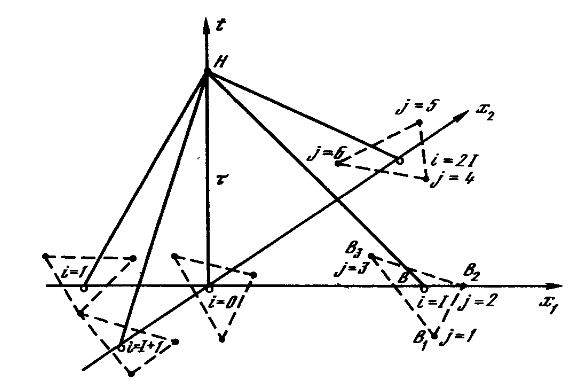
\includegraphics[width=0.6\textwidth]{png/characteristics-2d-triangles-inner.png}
\caption{Характеристики на неструктурированной сетке.}
\label{pic:gcm_2d}
\end{figure}

После того, как определён тетраэдр, в который попала характеристика, необходимо восстановить значение в точке пересечения характеристики со старым временным слоем. Для этого используется интерполяция значений в нужной точке по рассматриваемому тетраэдру.

Пусть искомая функция, задающая распределение в тетраэдре, является полиномом заданной степени $N$. Для линейной интерполяции (первый порядок точности по пространству) потребуется восстановить четыре коэффициента: постоянный член и множители перед $x, y, z$. Для квадратичной -- десять: те же четыре плюс еще шесть коэффициента перед $x^2, y^2, z^2, xy, xz, yz$. Для общего случая полинома степени $N$ количество коэффициентов в нем задается формулой $\frac{(N+1)(N+2)(N+3)}{6}$.

В произвольном тетраэдре $ABCD$ проведем плоскости, параллельные его сторонам, которые делят каждую из его сторон на $N$ частей (рис. \ref{pic:tetr-interpolation-base-points}). Количество точек внутри тетраэдра, в которых плоскости пересекаются между собой и со сторонами тетраэдраа, равно $\frac{(N+1)(N+2)(N+3)}{6}$. Именно эти точки пересечения мы выберем в качестве опорных, храня в них значения полинома, используемые для восстановления его величины во всех прочих точках.

\begin{figure}[h]
\centering
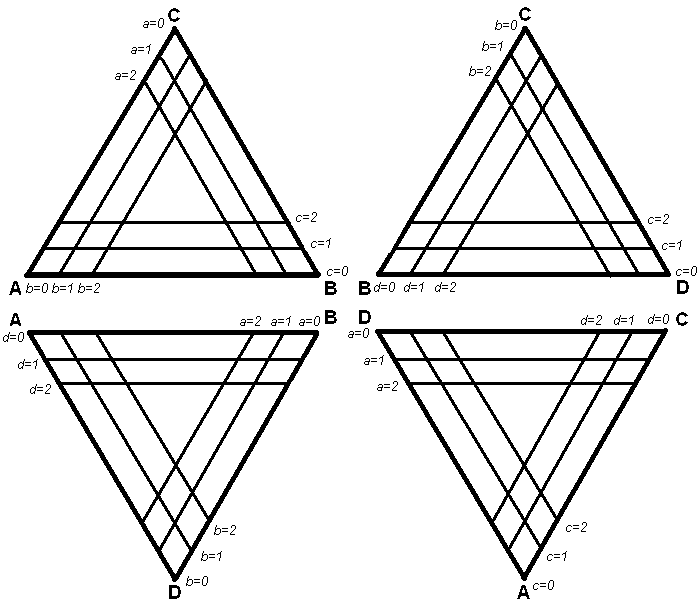
\includegraphics[width=0.5\textwidth]{png/tetr-interpolation-base-points.png}
\caption{Равномерное распределение опорных точек в тетраэдре (изображены стороны тетраэдра с проекциями плоскостей и их нумерацией).}
\label{pic:tetr-interpolation-base-points}
\end{figure}

Обозначим координаты вершин тетраэдра символами $\vec{r_A}, \vec{r_B}, \vec{r_C}, \vec{r_D}$, а ссылаться на опорные точки будем при помощи $r_{abcd}$. Индекс состоит из четырёх частей, каждая из которых описывает место пересечения плоскости, проходящей через опорную точку и параллельной определённой стороне, с соответствующим ребром тетраэдра (рис. \ref{pic:tetr-interpolation-base-points}). Для индексов любой опорной точки справедливо $a \ge 0, b \ge 0, c \ge 0, d \ge 0, a+b+c+d = N$.

Координаты опорной точки $r_{abcd}$ могут быть выражены через координаты вершин тетраэдра с использованием любой тройки индексов из четырех, достаточно взять систему координат с центром в одной из вершин и осями, проходящими через 3 другие.

Пусть необходимо реконструировать значение функции в произвольной точке $\vec{r}$ (обозначим её буквой $F$), которая может находиться как внутри тетраэдра, так и за его пределами. Введём в рассмотрение объёмы четырёх тетраэдров, которые формируются гранями исходного тетраэдра $ABCD$ и отрезками, соединяющими его вершины с точкой $F$.

Обозначим $V_i$ площадь того тетраэдра, одной из граней которого является грань исходного тетраэдра $ABCD$, противоположная его вершине $i$. Если $\vec{r}$ лежит внутри $ABCD$, то все четыре объёма $V_i$ положительны, в противном случае один или два «объёма» могут быть отрицательными. Но даже в этом случае, независимо от положения $\vec{r}$, их сумма будет равна объёму тетраэдра $ABCD$. Введём также относительные объёмы тех же тетраэдров $\nu_i = V_i / V$, где $V$ -- объём тетраэдра $ABCD$. Величины этих объёмов для точки $\vec{r}$, лежащей внутри $ABCD$, могут изменяться от нуля до единицы.

Значение функции в искомой точке $\phi(\vec{r})$ необходимо выразить через значения $\phi_{abcd} = \phi(r_{abcd})$, которые она принимает в опорных точках:
\begin{equation}
\phi(\vec{r}) = \sum_{a,b,c,d}{w_{abcd}(\vec{r}) \phi_{abcd}},
\end{equation}
где $w_{abcd}(\vec{r})$ -- вес опорной точки $\vec{r_{abcd}}$, также являющийся полиномом степени $N$. Вес обращается в единицу в одной опорной точке и в ноль во всех остальных опорных точках. Следующая функция веса удовлетворяет поставленным условиям:
\begin{equation}
w_{abcd}(\vec{r}) = \frac{ \prod_{i=1}^N{\nu_{T_i}(r) - \frac{n_i}{N}} }{ \prod_{i=1}^N{\nu_{T_i}(r_{abcd}) - \frac{n_i}{N}} }, \textrm{ где } T_i \in \{A, B, C, D\}, 0 \le n_i \le N
\end{equation}
при условии правильного подбора величин ${T_i}, {n_i}$. Принципиально, что если индексы двух опорных точек совпадают с точностью до перестановки, то функции их весов совпадают с точностью до той же перестановки величин в ${T_i}$.

\paragraph{Интерполяция первого порядка.} Опорные точки для линейной интерполяции -- $r_{1000}, r_{0100}, r_{0010}, r_{0001}$ (рис. \ref{pic:tetr-interpolation-1st-order-1}).

\begin{figure}[h]
\centering
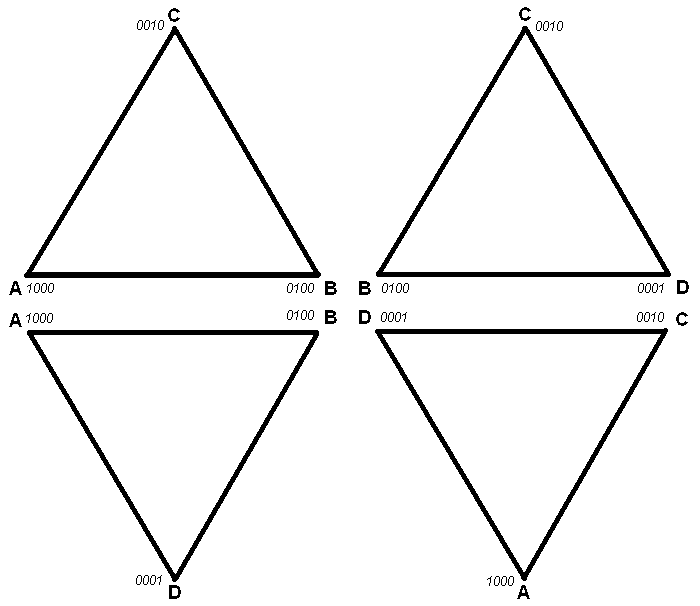
\includegraphics[width=0.5\textwidth]{png/tetr-interp-1st-order-1.png}
\caption{Опорные точки для интерполяции первого порядка.}
\label{pic:tetr-interpolation-1st-order-1}
\end{figure}

Найдём $w_{1000}(r)$ (рис. \ref{pic:tetr-interpolation-1st-order-2}):
\begin{equation}
w_{1000}(r) = \frac{ \nu_{T_1}(r) - n_1 }{ \nu_{T_1}(r_{1000}) - n_1 }.
\end{equation}

\begin{figure}[h]
\centering
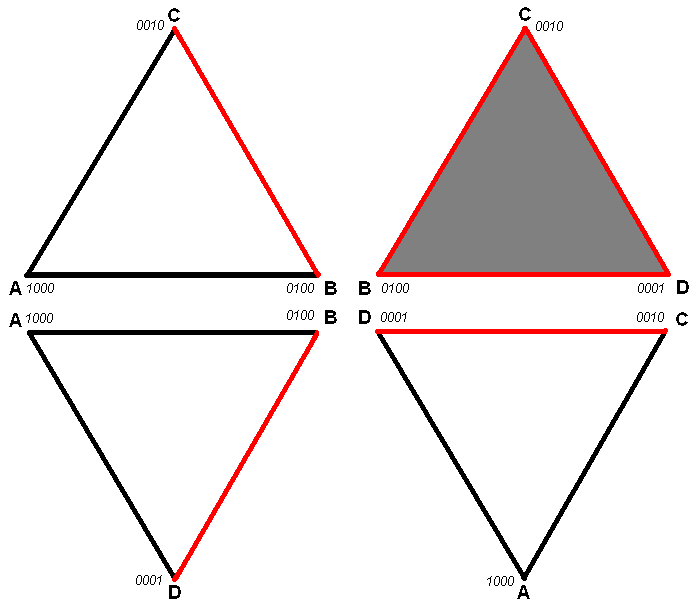
\includegraphics[width=0.5\textwidth]{png/tetr-interp-1st-order-2.png}
\caption{К вычислению весов для интерполяции первого порядка.}
\label{pic:tetr-interpolation-1st-order-2}
\end{figure}

Пусть $r = r_{0001}$. Подбираем $T_1$ и $n_1$:
\begin{align}
0 = \frac{ \nu_{T_1}(r_{0001}) - n_1 }{ \nu_{T_1}(r_{1000}) - n_1 } = \frac{ \nu_{A}(r_{0001}) - n_1 }{ \nu_{A}(r_{1000}) - n_1 } = \frac{0-n_1}{1-n_1} = \frac{0-0}{1-0} = \nu_{A}(r_{0001}).
\end{align}

Выполнив аналогичную процедуру для остальных весов, получаем:
\begin{align}
w_{1000}(r) = \nu_{A}(r) & & w_{0100}(r) = \nu_{B}(r), \nonumber\\
w_{0010}(r) = \nu_{C}(r) & & w_{0001}(r) = \nu_{D}(r).
\end{align}


\paragraph{Интерполяция второго порядка.} Опорные точки для квадратичной интерполяции -- $r_{2000}, r_{0200}, r_{0020}, r_{0002}, r_{1100}, r_{0110}, r_{0011}, r_{1001}, r_{1010}, r_{0101}$ (рис. \ref{pic:tetr-interpolation-2nd-order-1}).

\begin{figure}[h]
\centering
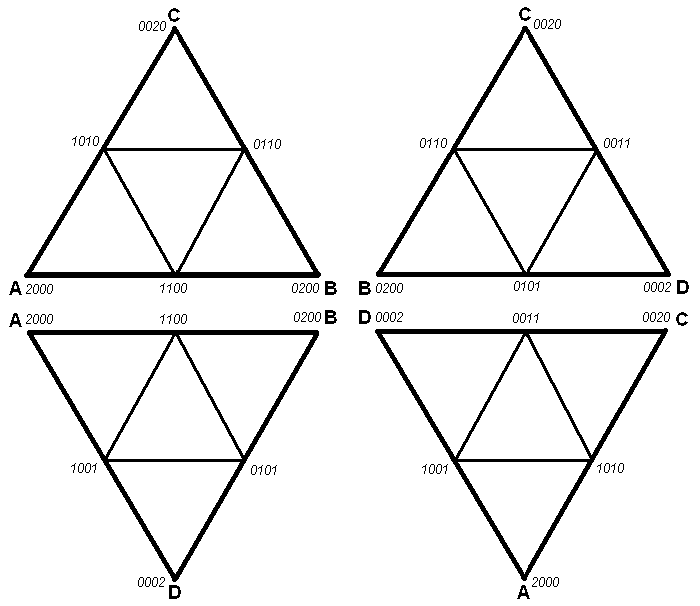
\includegraphics[width=0.5\textwidth]{png/tetr-interp-2nd-order-1.png}
\caption{Опорные точки для интерполяции второго порядка.}
\label{pic:tetr-interpolation-2nd-order-1}
\end{figure}


Найдём $w_{2000}(r)$:
\begin{equation}
w_{2000}(r) = \frac{ \nu_{T_1}(r) - \frac{n_1}{2} }{ \nu_{T_1}(r_{2000}) - \frac{n_1}{2} } \frac{ \nu_{T_2}(r) - \frac{n_2}{2} }{ \nu_{T_2}(r_{2000}) - \frac{n_2}{2} }.
\end{equation}


Пусть $r = r_{0002}$. Подбираем $T_1$ и $n_1$ (см. рис. \ref{pic:tetr-interpolation-2nd-order-2}а).

\begin{align}
0 = \frac{ \nu_{T_1}(r_{0002}) - \frac{n_1}{2} }{ \nu_{T_1}(r_{2000}) - \frac{n_1}{2} } = \frac{ \nu_{A}(r_{0002}) - \frac{n_1}{2} }{ \nu_{A}(r_{2000}) - \frac{n_1}{2} } = \frac{ 0 - \frac{n_1}{2} }{ 1 - \frac{n_1}{2} } = \frac{ 0 - \frac{0}{2} }{ 1 - \frac{0}{2} } = \nu_{A}(r_{0002}).
\end{align}

Таким образом, первый множитель $\nu_{A}(r)$.

Пусть $r = r_{1100}$. Подбираем $T_2$ и $n_2$ (см. рис. \ref{pic:tetr-interpolation-2nd-order-2}б).

\begin{align}
0 = \frac{ \nu_{T_2}(r_{1100}) - \frac{n_2}{2} }{ \nu_{T_2}(r_{2000}) - \frac{n_2}{2} } = \frac{ \nu_{A}(r_{1100}) - \frac{n_2}{2} }{ \nu_{A}(r_{2000}) - \frac{n_2}{2} } = \frac{ \frac{1}{2} - \frac{n_2}{2} }{ 1 - \frac{n_2}{2} } = \frac{ \frac{1}{2} - \frac{1}{2} }{ 1 - \frac{1}{2} } = 2\nu_{A}(r_{1100}) - 1.
\end{align}

Таким образом, второй множитель $2\nu_{A}(r)-1$.

Итого для веса $w_{2000}(r)$ получаем $w_{2000}(r) = \nu_{A}(r) (2\nu_{A}(r)-1)$. Остальные веса вершин тетраэдра получаются перестановкой индексов в данной формуле.

Найдём $w_{1100}(r)$:
\begin{equation}
w_{1100}(r) = \frac{ \nu_{T_1}(r) - \frac{n_1}{2} }{ \nu_{T_1}(r_{1100}) - \frac{n_1}{2} } \frac{ \nu_{T_2}(r) - \frac{n_2}{2} }{ \nu_{T_2}(r_{1100}) - \frac{n_2}{2} }.
\end{equation}

Пусть $r = r_{0002}$. Подбираем $T_1$ и $n_1$ (см. рис. \ref{pic:tetr-interpolation-2nd-order-2}в).

\begin{align}
0 = \frac{ \nu_{T_1}(r_{0002}) - \frac{n_1}{2} }{ \nu_{T_2}(r_{1100}) - \frac{n_1}{2} } = \frac{ \nu_{A}(r_{0002}) - \frac{n_1}{2} }{ \nu_{A}(r_{1100}) - \frac{n_1}{2} } = \frac{ 0 - \frac{n_1}{2} }{ \frac{1}{2} - \frac{n_1}{2} } = \frac{ 0 - \frac{0}{2} }{ \frac{1}{2} - \frac{0}{2} } = 2\nu_{A}(r_{0002}).
\end{align}

Таким образом, первый множитель $2\nu_{A}(r)$.

Пусть $r = r_{2000}$. Подбираем $T_2$ и $n_2$ (см. рис. \ref{pic:tetr-interpolation-2nd-order-2}г).

\begin{align}
0 = \frac{ \nu_{T_2}(r_{2000}) - \frac{n_2}{2} }{ \nu_{T_2}(r_{1100}) - \frac{n_2}{2} } = \frac{ \nu_{B}(r_{2000}) - \frac{n_2}{2} }{ \nu_{B}(r_{1100}) - \frac{n_2}{2} } = \frac{ 0 - \frac{n_2}{2} }{ \frac{1}{2} - \frac{n_2}{2} } = \frac{ 0 - \frac{0}{2} }{ \frac{1}{2} - \frac{0}{2} } = 2\nu_{B}(r_{2000}).
\end{align}

Таким образом, второй множитель $2\nu_{B}(r)$.

Итого для веса $w_{1100}(r)$ получаем $w_{1100}(r) = 4 \nu_{A}(r) \nu_{B}(r)$. Остальные веса дополнительных вершин получаются перестановкой индексов в данной формуле.



\begin{figure}[h]
\begin{subfigure}[b]{0.5\textwidth}
\centering
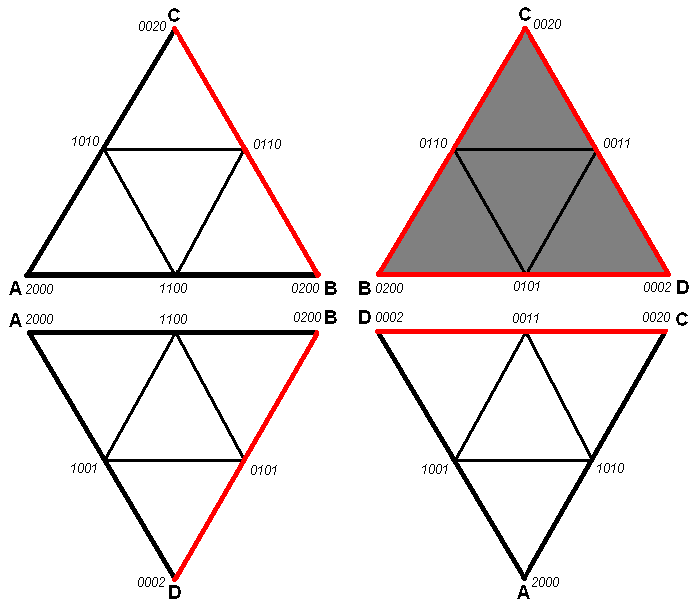
\includegraphics[width=\textwidth]{png/tetr-interp-2nd-order-2.png}
\caption{Схема для $w_{2000}(r)$ и $r = r_{0002}$}
\end{subfigure}
\begin{subfigure}[b]{0.5\textwidth}
\centering
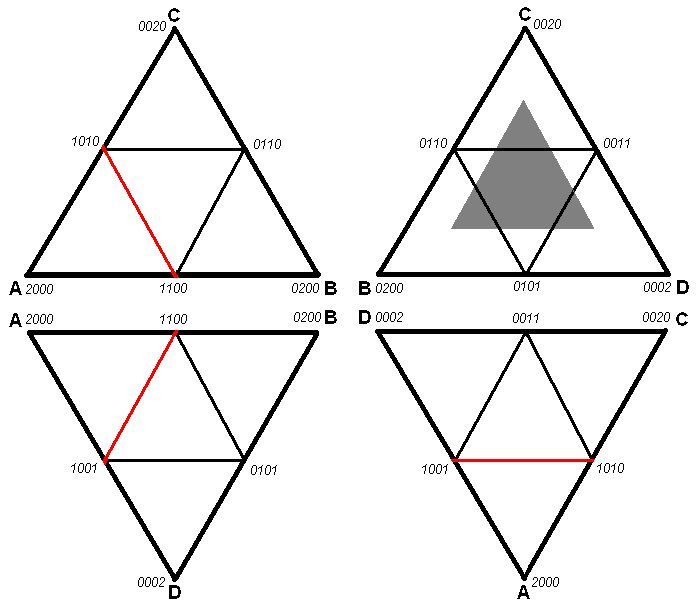
\includegraphics[width=\textwidth]{png/tetr-interp-2nd-order-3.png}
\caption{Схема для $w_{2000}(r)$ и $r = r_{1100}$}
\end{subfigure}
\begin{subfigure}[b]{0.5\textwidth}
\centering
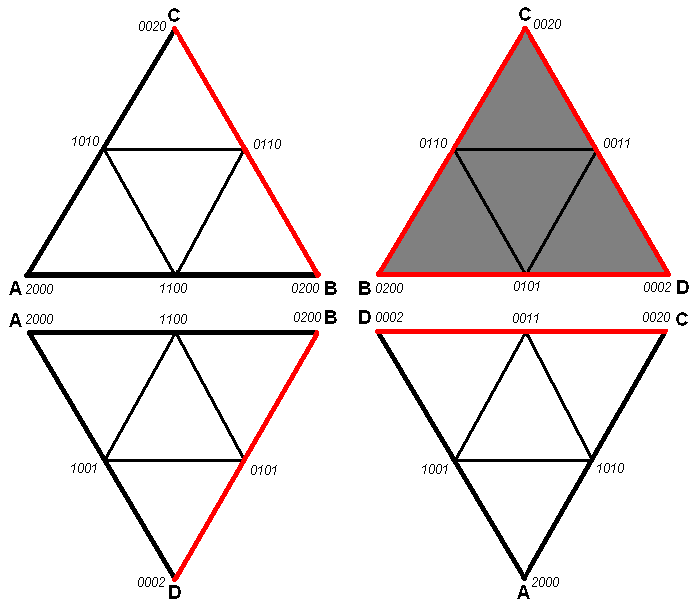
\includegraphics[width=\textwidth]{png/tetr-interp-2nd-order-4.png}
\caption{Схема для $w_{1100}(r)$ и $r = r_{0002}$}
\end{subfigure}
\begin{subfigure}[b]{0.5\textwidth}
\centering
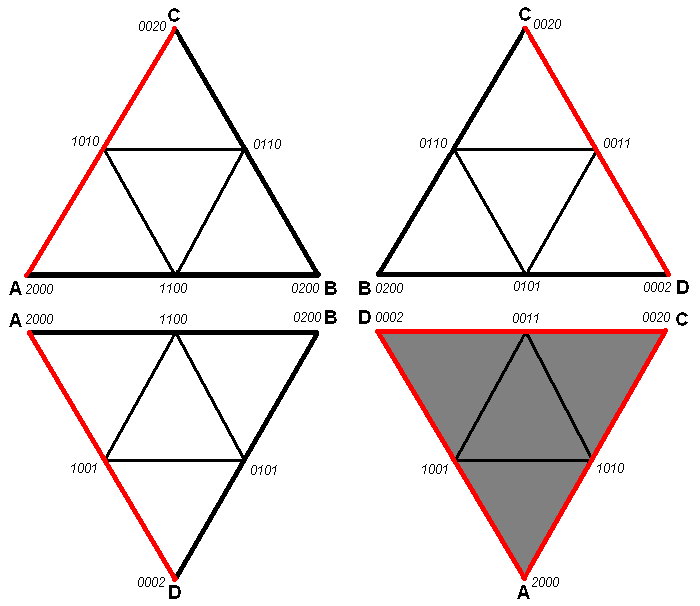
\includegraphics[width=\textwidth]{png/tetr-interp-2nd-order-5.png}
\caption{Схема для $w_{1100}(r)$ и $r = r_{2000}$}
\end{subfigure}
\caption{К вычислению весов для интерполяции второго порядка.}
\label{pic:tetr-interpolation-2nd-order-2}
\end{figure}

Итоговые веса для интерполяции второго порядка:
\begin{flalign}
w_{2000}(r) &=& \nu_{A}(r) (2\nu_{A}(r)-1) & & & w_{0200}(r) &=& \nu_{B}(r) (2\nu_{B}(r)-1), &\nonumber\\
w_{0020}(r) &=& \nu_{C}(r) (2\nu_{C}(r)-1) & & & w_{0002}(r) &=& \nu_{D}(r) (2\nu_{D}(r)-1), &\nonumber\\
w_{1100}(r) &=& 4 \nu_{A}(r) \nu_{B}(r) & & & w_{0110}(r) &=& 4 \nu_{B}(r) \nu_{C}(r), &\nonumber\\
w_{0011}(r) &=& 4 \nu_{C}(r) \nu_{D}(r) & & & w_{1001}(r) &=& 4 \nu_{D}(r) \nu_{A}(r), &\nonumber\\
w_{1010}(r) &=& 4 \nu_{A}(r) \nu_{C}(r) & & & w_{0101}(r) &=& 4 \nu_{B}(r) \nu_{D}(r). &
\end{flalign}


\paragraph{Интерполяция более высоких порядков.} Формулы для интерполяции более высоких порядков строятся аналогично. В данной работе используются схемы первого и второго порядка, поэтому вывод для более высоких порядков не приводится.

\paragraph{Гибридизация схемы.} Гибридная схема на неструктурированной сетке строится принципиально так же, как для структурированной. Используются две опорные схемы -- разобранные выше схемы с интерполяцией первого и второго порядка. В зависимости от локальной гладкости численного решения происходит переключение между схемами -- на гладких участках используется схема второго порядка, в области разрывов происходит переключение на схему первого порядка.


\subsubsection{Расчёт граничных узлов}

%\todo{Внятно написать эти два раздела}

Описанный метод подходит для расчёта внутренних узлов
сетки, т.е. только в том случае, если все характеристики, выпущенные из узла, не
выводит за пределы области интегрирования. В случае, когда узел находится на границе расчётной области, 
применяется иной подход для решения задачи. Рассматриваемая система
уравнений в граничных узлах области интегрирования имеет ровно три
\cite{chelnokov} выводящие характеристики. Поэтому для корректной постановки
задачи требуется задание граничных условий для каждого внешнего узла сетки в
количестве, равном числу выводящих характеристик. 

Граничные условия могут быть различными. В данной работе используется ряд граничных условий.

Свободная граница:
\begin{align}
\sigma_\tau=\sigma_n=0.
\end{align}
Здесь $\sigma_n$ и $\sigma_\tau$ -- нормальное и тангенциальное напряжение в граничной точке.

Заданная внешняя сила:
\begin{align}
\sigma_\tau &= \sigma_{\tau 0}, \nonumber\\
\sigma_n &= \sigma_{n 0}
\end{align}
Здесь $\sigma_{n 0}$ и $\sigma_{\tau 0}$ -- заданные извне нормальное и тангенциальное напряжение в граничной точке.

Заданная скорость границы:
\begin{align}
\vec{v} = \vec{v_0}.
\end{align}
Здесь $\vec{v_0}$ -- заданный извне вектор скорости в точке границы.


\subsubsection{Расчёт контактных узлов}

Расчёт контактной границы между двумя телами в целом аналогичен расчёту границы тела. Однако, в точке контакта присутствуют два узла -- по одному из каждого контактирующего тела. В каждом из них 6 уравнений исходной системы корректны, а 3 несовместны, так как соответствуют выводящим характеристикам. Кроме того, так как тела контактируют, для значений функции в двух рассматриваемых узлах есть уравнений связей. Уравнения связей должны задавать 6 условий, чтобы компенсировать 3 несовместные уравнения в каждом узле.

В результате получается система из 18 уравнений (6 у каждого узла и 6 уравнений связей) с 18 неизвестными (по 9 в каждом узле). Решая эту систему, получаем согласованные значения функции в обоих контактирующих узлах.

Уравнения связей могут быть различными, задавая различные условия контакта. В данной работе используется ряд контактных условий.

Скольжение тел друг относительно друга:
\begin{align}
v_n&=\tilde{v}_n,\nonumber\\
\sigma_n&=\tilde{\sigma}_n,\nonumber\\
\sigma_\tau&=\tilde{\sigma}_\tau=0.
\end{align}
Здесь $\sigma_n$ и $\sigma_\tau$ -- нормальное и тангенциальное напряжение в граничной точке. Символы с чертой относятся к первому телу, без черты -- ко второму.

Слипание тел:
\begin{align}
v_n&=\tilde{v}_n,\nonumber\\
v_\tau&=\tilde{v}_\tau.
\end{align}


\clearpage
\newpage

\subsection{Решение многомерной задачи}

\subsubsection{Схема с расщеплением по направлениям}

Система \ref{matrix_equation} (или что то же самое \ref{matrix_equation_generalized}) позволяет построить схему для решения трёхмерной задачи, если построены и исследованы одномерные схемы для задач:
\begin{equation}
\frac{\partial\vec{u}}{\partial{t}} + \mathbf{A}_{\xi_j} \frac{\partial\vec{u}}{\partial{\xi_j}} = 0.
\end{equation}

Такой подход называется расщеплением по направлениям и был предложен Р.П. Федоренко (\cite{fedorenko}). Идея метода решения исходной задачи состоит в замене исходной системы уравнений \ref{matrix_equation} одномерными системами -- тремя в случае отсутствия в исходной системе правой части и четырьмя, если правая часть имеется:
\begin{equation}
\frac{\partial}{\partial t}\vec u+\mathbf{A}_x \frac{\partial}{\partial x}\vec u = 0,
\label{matrix_equation_x}
\end{equation}
\begin{equation}
\frac{\partial}{\partial t}\vec u+\mathbf{A}_y \frac{\partial}{\partial y}\vec u = 0,
\label{matrix_equation_y}
\end{equation}
\begin{equation}
\frac{\partial}{\partial t}\vec u+\mathbf{A}_z \frac{\partial}{\partial z}\vec u = 0,
\label{matrix_equation_z}
\end{equation}
\begin{equation}
\frac{\partial}{\partial t}\vec u = \vec f.
\label{matrix_equation_f}
\end{equation}

Обозначим $F(\mathbf A_{\xi_1}, \mathbf A_{\xi_2}, \mathbf A_{\xi_3}, \vec f)$ оператор перехода между временными слоями $n$ и $n+1$, а $F_j(\mathbf A_{\xi_j}), j=1..3$ и $F_j(\vec f), j=4$ -- оператор, соответствующий $j$-ому уравнению в расщеплённой системе.

Необходимо сконструировать оператор $F$ из операторов $f_j, j=1..4$, обеспечив при этом аппроксимацию и устойчивость итоговой схемы, а также приемлемую вычислительную сложность алгоритма при его реализации.

Как разобрано выше, для каждой одномерной задачи существует ограничение на шаг по времени
\begin{equation}
\tau_j \le \frac{\min(h)}{\max(|\lambda_j|)},
\end{equation}

где $\min(h)$ -- минимальная высота тетраэдра в сетке, а $\max(|\lambda_j|)$ -- максимальное по модулю собственное число матрицы $\mathbf A_{\xi_j}$. Теоретически, в этом соотношении можно заменить $\min(h)$ на $\min(h_j)$ -- минимальное расстояние в направлении $j$-ой оси координат от узла сетки до точки пересечения с ближайшей гранью соседнего тетраэдра. Это расстояние может быть несколько больше, чем абсолютный минимум высоты по сетке $\min(h)$, и за счет этого обеспечивать несколько больший допустимый шаг по времени. Однако, на практике в силу случайной ориентации как тетраэдров сетки, так и координатных осей, потенциальное преимущество мало и не стоит того, чтобы усложнять алгоритм расчёта как логически из-за добавления новых элементов, так и вычислительно из-за необходимости постоянно определять новые точки пересечения.

При выполнении условия на $\tau_j$ схема, соответствующая оператору $F_j$, устойчива и имеет свой порядок аппроксимации по времени и пространству для одномерной задачи. Теперь рассмотрим различные варианты составления оператора $F$ из $F_j$.


\subsubsection{Схема с расщеплением первого порядка}

В простейшем случае можно сложить операторы $F_j$ с коэффициентами $a_j$. При таком подходе получаем:
\begin{align}
F(\mathbf A_{\xi_1}, \mathbf A_{\xi_2}, \mathbf A_{\xi_3}, \vec f) &= \sum\limits_{j} a_j F_j(\frac{1}{a_j} \mathbf A_{\xi_j}), \nonumber\\
\sum\limits_{j} a_j &= 1, \nonumber\\
a_j &> 0.
\end{align}

Такая схема обеспечивает первый порядок аппроксимации итогового оператора $F$, если в качестве $F_j$ были выбраны схемы как минимум первого порядка. В выборе $a_j$ присутствует определённый произвол, что позволяет использовать их для получения максимального шага по времени.

Действительно, собственные числа матриц $\mathbf A_{\xi_j}^* = \frac{1}{a_j} \mathbf A_{\xi_j}$ будут в $a_j$ раз отличаться от собственных чисел исходных матриц $\mathbf A_{\xi_j}$. Максимально допустимый шаг по времени
\begin{equation}
\tau \le \max{\tau_j} = \frac{\min(h)}{\max(|\lambda_j^*|)} = \frac{\min(h)a_j}{\max(|\lambda_j|)}.
\end{equation}

Таким образом, для максимизации допустимого шага получаем условие:
\begin{equation}
\frac{a_1}{\max(|\lambda_1|)} = \frac{a_2}{\max(|\lambda_2|)} = \frac{a_3}{\max(|\lambda_3|)}.
\end{equation}

Откуда следует
\begin{align}
a_j = \frac{\max(|\lambda_j|)}{\max(|\lambda_1|)+\max(|\lambda_2|)+\max(|\lambda_3|)},\nonumber\\
\tau = \frac{\min(h)}{\max(|\lambda_1|)+\max(|\lambda_2|)+\max(|\lambda_3|)}
\end{align}

Видно, что при таком конструировании расщепления получается вычислительно простой алгоритм -- требуется только вычислить независимое воздействие операторов $F_j$ на временном слое $n$, чтобы потом получить значение на временном слое $n+1$ как их сумму. Однако, схема обеспечивает только первый порядок аппроксимации $F$, даже если отдельно $F_j$ имеют более высокий порядок. Кроме того, допустимый шаг по времени заметно уменьшается (как правило, в 3 раза, так как $\max(|\lambda_j|)$ одинаково для всех матриц $\mathbf A_{\xi_j}$.


\subsubsection{Схема с расщеплением второго порядка}

Для обеспечения второго порядка аппроксимации итоговой схемы необходимо операторы $F_j$ не сложить, а перемножить
\begin{align}
\label{split_scheme_2nd_order}
F(\mathbf A_{\xi_1}, \mathbf A_{\xi_2}, \mathbf A_{\xi_3}, \vec f) = F_1(\mathbf A_{\xi_1}) F_2(\mathbf A_{\xi_2}) F_3(\mathbf A_{\xi_3}).
\end{align}

С точки зрения реализации это означает, что сначала к значениям на временном слое $n$ применяется первый оператор, потом к результату действия первого оператора -- второй, к результату второго -- третий. Значения, полученные после применения всех операторов, являются значениями на новом временном слое $n+1$:
\begin{align}
\vec u^{'} &= F_1(\mathbf A_{\xi_1}) \vec u^n, \nonumber\\
\vec u^{''} &= F_2(\mathbf A_{\xi_2}) \vec u^{'}, \nonumber\\
\vec u^{n+1} &= F_3(\mathbf A_{\xi_3}) \vec u^{''}.
\end{align}

Допустимый шаг по времени определяется минимальным допустимым шагом по времени для схем $F_j$:
\begin{align}
\tau = \min\limits_{j}(\tau_j) = \min\limits_{j}(\frac{\min(h)}{\max(|\lambda_j|)}) = \frac{\min(h)}{\max\limits_{j}\max(|\lambda_j|)}.
\end{align}

Таким образом, расщепление данного вида обеспечивает второй порядок аппроксимации и не приводит к уменьшению допустимого шага по времени. Однако, если использовать схему в виде \ref{split_scheme_2nd_order}, то очевидным образом возникает несимметрия решения, так как направления координатных осей перестают быть равноправными.

Метод симметризации схемы достаточно очевиден -- необходимо использовать не одно произведение операторов, которое порождает выделенные направления, а усреднять все возможные перестановки операторов $F_j$:
\begin{align}
\label{split_scheme_2nd_order_sym}
F(\mathbf A_{\xi_1}, \mathbf A_{\xi_2}, \mathbf A_{\xi_3}, \vec f) = \frac{1}{6} \sum\limits_{i \ne j \ne k} F_i(\mathbf A_{\xi_i}) F_j(\mathbf A_{\xi_j}) F_k(\mathbf A_{\xi_k}).
\end{align}

Такая схема становится симметричной, но теперь приходится считать действие операторов $F_j$ 18 раз вместо 3 раз.


\subsubsection{Схема с расщеплением и случайным выбором базиса}

Альтернативным способом симметризации схемы \ref{split_scheme_2nd_order} является случайный выбор базиса. В этом случае схема расщепления обеспечивает второй порядок аппроксимации многомерной задачи и возможность использовать большое значение $\tau$. Случайный выбор базиса обеспечивает отсутствие выделенных направлений и симметричность решения. За счет этого на каждом временном шаге требуется вычислять только 3 оператора $F_j$.

Обратной стороной такого подхода, который проявляется при практической реализации метода, является тот факт, что в случайно выбранном базисе из-за изменения направлений осей постоянно меняются точки на предыдущем временном слое, в которые попадают характеристики и по которым производится реконструкция решения. В результате требуется искать эти точки заново после смены базиса на каждом шаге. Однако, при разумной организации структур данных, вычислительная сложность этой операции достаточно невелика и такой подход оказывается значительно экономичнее, чем вычисление операторов $F_j$ дополнительные 15 раз.

\clearpage
\newpage

\subsection{Движение сетки}

%\todo{Переписать слова ниже. Объяснить внятно про конвективные члены.}

В случае конечных деформаций существует несколько подходов к описанию движения точек среды.

Эйлерова сетка строится однократно и в дальнейшем не изменяется. Это может быть наилучшим решением для тел с фиксированными границами. Для решения задач с конечными деформациями границ выбирают наиболее простую форму эйлеровой сетки — декартову решетку, потому что, независимо от формы ячеек, неподвижные узлы и ребра сетки не будут совпадать в каждый момент времени с движущимися границами, и неизбежны сложности, описанные для декартовых решеток.

Точки лагранжевой сетки смещаются вместе с точками тела, поэтому границы тела всегда совпадают с сеточными линиями. Однако при наличии сдвиговых деформаций в теле, ячейки лагранжевой сетки могут постепенно вырождаться и пересекать друг друга. Численные методы при вырождении сетки обнаруживают неустойчивость и счет приходится прекращать. Поэтому неизбежен подход, называемый лагранжева сетка с перестройкой, в котором, как только детектируется приближение сетки к вырожденному состоянию, производится построение новой сетки, а значения в новых узлах интерполируются из прежних значений. Процедура интерполяции сама по себе приводит к потере точности решения, поэтому желательно перестраивать сетку как можно реже. Ниже будет предложен альтернативный способ решения проблемы больших деформаций, который вместо перестроения сетки использует динамический выбор сеточного шаблона в зависимости от локальных свойств решения.

Подвижная сетка является обобщением лагранжевой, ее точки движутся от слоя к слою с ненулевыми скоростями и смещаются как относительно неподвижной системы координат, так и относительно точек тела. Их движение может быть подобрано таким образом, чтобы исключить вырождение сетки со временем. Однако использование подвижной сетки требует вносить изменения в решаемые уравнения для учета конвективных членов.

Расчет на лагранжевой сетке из тетраэдров подразумевает, что скорость смещения вершин сетки совпадает со скоростью среды. Но в методах второго порядка и выше вводятся дополнительные узлы, отличные от вершин, движение которых задается линейной интерполяцией движений вершин тетраэдра, в котором они расположены. Даже если скорость всех вершин является лагранжевой, то узлы, не совпадающие с вершинами, смещаются относительно точек среды. Это означает, что при их расчете необходимо учитывать конвективные члены. Отличие скорости этих узлов от скорости среды невелико: $O(h^2)$, где $h$ — мелкость сетки. Собственные значения матриц при поправке на конвекцию также изменятся на $O(h^2)$.

Отличие мест пересечения характеристики до и после поправки со слоем $t^n$ составит $\tau O(h^h2) = O(\tau^3)$, такого же порядка и отличие в восстанавливаемом интерполяцией решении. Поэтому в методе второго порядка можно не рассматривать отличие движения узлов в центре ребер от лагранжевых — это не понизит степень аппроксимации, а в методах третьего порядков и выше поправка необходима.

\clearpage
\newpage

\subsection{Выделение контактных границ}

При взаимном движении тел, а также в задачах с конечными деформациями отдельной задачей становится построение алгоритма явного выделения контактных границ. Стандартный подход (именно он использован в этой работе) к реализации состоит из двух этапов:
\begin{itemize}
	\item грубое (см. рис. \ref{pic:collision_detection}) определение областей потенциально возможного контакта при помощи AABB\footnote{AABB (Axis-aligned bounding box) -- ограничивающий параллелепипед, выровненный по осям };
	\item уточнение контактирующих узлов внутри найденных областей.
\end{itemize}
\begin{figure}[htp]
\centering
\includegraphics[width=0.6\textwidth]{eps/collision_detection.eps}
\caption{Использование AABB для грубого определения областей контакта. На
рисунке изображены тела $B_1$ и $B_2$, а также AABB, построенные для контуров
$C_1$ и $C_2$ этих тел. Контакты ищутся в пересечении разных AABB.}
\label{pic:collision_detection}
\end{figure}
По пересечению AABB определяются пары <<потенциально>> находящихся в контакте тел. Затем для каждой найденной пары проводится уточнение зоны контакта: проверяются <<на контакт>> все пары узлов одного тела и треугольников поверхности другого. Пары <<контактирующих>> узлов и треугольников определяются полным перебором по <<кандидатов>>, попавших внутрь пересечения AABB. Под контактом точки и треугольника здесь понимается следующее: считаем, что треугольник и точка контактируют, если зона влияния (сфера заранее выбранного радиуса) точки пересекает треугольник (см. рис. \ref{pic:contact_detection}).
\begin{figure}[htp]
\centering
\includegraphics[width=0.6\textwidth]{pdf/contact_detection.pdf}
\caption{Определение контакта.}
\label{pic:contact_detection}
\end{figure}
Если треугольник и точка находятся в контакте, то следующим шагом строится парный виртуальный узел -- этот узел лежит внутри контактирующего треугольника так, чтобы прямая проходящая через реальный и виртуальный узлы, являлась нормалью к треугольнику (см. рис. \ref{pic:contact_processing}).
\begin{figure}[htp]
\centering
\includegraphics[width=0.6\textwidth]{pdf/contact_processing.pdf}
\caption{Построение виртуальных узлов при обработке контактирующих границ.}
\label{pic:contact_processing}
\end{figure}
После того, как виртуальный узел построен, получаются значения всех величин в нём. Для этого в данной работе использовалась линейная интерполяция при помощи барицентрических координат. Задача заключается в следующем (см. рис. \ref{pic:triangle_interpolation}): есть треугольник и точка, лежащая в его плоскости, в трёхмерном пространстве, нужно, используя известные значения в вершинах треугольника, определить значение в точке.
\begin{figure}[htp]
\centering
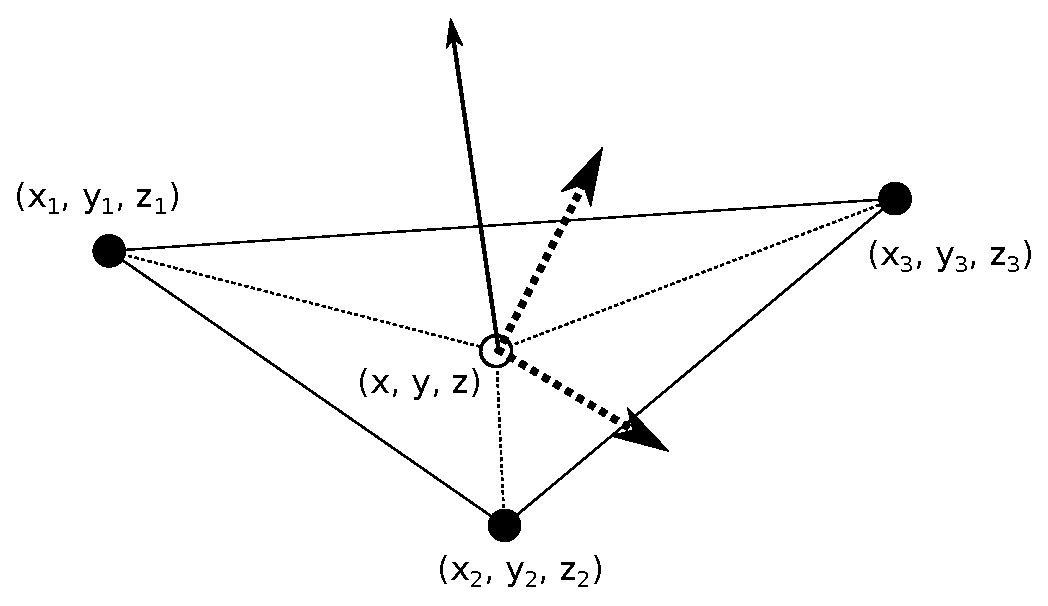
\includegraphics[width=0.6\textwidth]{eps/triangle_interpolation.eps}
\caption{Выбор новых осей координат при интерполяции в треугольнике.}
\label{pic:triangle_interpolation}
\end{figure}
В работе используется следующий подход для реализации интерполяции:
\begin{itemize}
	\item поворотом осей координат добиваемся того, чтобы все четыре точки имели одинаковую координату $\tilde{x}$;
	\item используем интерполяцию в плоскости через барицентрические координаты.
\end{itemize}
Пусть $\vec{n}=(n_1,n_2,n_3)$ -- нормаль к плоскости треугольника, тогда в системе координат с базисными векторами:
\begin{align}
\label{eq:new_coords}
\vec{\tilde{e}}_1&=(n_1, n_2, n_3), \nonumber \\
\vec{\tilde{e}}_2&=(n_3, 0, -n_1), \nonumber \\
\vec{\tilde{e}}_3&=(n_1*n_2, -n_1^2-n_3^2, n_2*n_3)
\end{align}
все четыре точки имеют одинаковую координату $\tilde{x}$. Такую систему
координат невозможно использовать, если $n_1=n_3=0$, но в этом случае все точки
имеют одинаковую координату $y$, поэтому, сделав замену
\begin{align}
\label{eq:new_coords_2}
\tilde{x}&=y \nonumber\\
\tilde{y}&=x \nonumber \\
\tilde{z}&=z,
\end{align}
придём опять к ситуации, когда все четыре точки имеют одинаковую координату $x$.
После этих преобразований значение в точке $(x,y,z)$ может быть вычислено по формуле
\begin{equation}
\label{eq:triangle_interpolation}
v=v_1*\lambda_1+v_2*\lambda_2+v_3*\lambda_3, 
\end{equation}
где $v_1,v_2,v_3$ -- значения в вершинах треугольника, а $\lambda_1,\lambda_2,\lambda_3$ -- барицентрические координаты
\begin{align}
\label{eq:barycentric_coords}
\lambda_1&=\frac{(y_2-y_3)(x-x_3)+(x_3-x_2)(y-y_3)}{(y_2-y_3)(x_1-x_3)+(x_3-x_2)(y_1-y_3)}, \nonumber \\
\lambda_2&=\frac{(y_3-y_1)(x-x_3)+(x_1-x_3)(y-y_3)}{(y_2-y_3)(x_1-x_3)+(x_3-x_2)(y_1-y_3)}, \nonumber \\
\lambda_3&=1-\lambda_1-\lambda_2.
\end{align}
Эта интерполяция обладает первым порядком точности, что согласуется с порядком точности остальных частей алгоритма.


\clearpage
\newpage


\subsection{Расчёт с шагом $\tau > h/\lambda$}

\subsubsection{Необходимость расчёта с шагом $\tau > h/\lambda$}

Одной из принципиальных проблем, с которыми сталкивается метод характеристик на сетках из тетраэдров при попытке расчета им реальных задач, является низкое качество сеток, создаваемых стандартными генераторами сеток. Данный вопрос практически всегда остается за рамками в любых публикациях по теме сеточно-характеристических методов, так как не связан непосредственно с конструированием самого метода. Тем не менее, для практики эта проблема крайне важна, поэтому остановимся на ней подробнее.

Если подходить к вопросу формально, то сеточно-характеристический метод может использоваться на любой сетке из тетраэдров. Однако, как было рассмотрено выше, для сеток из тетраэдров имеет место ограничение на шаг по времени, аналогичное курантовскому шагу для равномерной прямоугольной сетки. Так для каждого узла сетки:

\begin{equation}
\tau \le \frac{\min(h)}{\max(|\lambda|)},
\end{equation}

где $\min(h)$ -- минимальная высота тетраэдра, в которые входит данный узел, $\max(|\lambda|)$ -- максимальное по модулю собственное число матрицы $\mathbf A$ для данного узла.

С практической точки зрения крайне нежелательна ситуация, когда $\tau$ оказывается малым для отдельных узлов сетки, так как это накладывает ограничения на шаг по времени для всей сетки. Разумеется, необходимо различать случай, когда малый шаг по времени продиктован объективными требованиями высокого разрешения по времени и пространству, и случай, когда он является нежелательным следствием тех или иных проблем. В данный момент мы сосредоточимся на втором случае.

В таблице \ref{tbl:mesh-stats-summary} приведены данные по сеткам из тетраэдров, созданных в кубе с ребром 10 с помощью различных генераторов. Во всех случаях было задано значение мелкости сетки $h_* = 0.25$. В идеальном случае была бы построена сетка из правильных тетраэдров одинакового размера с высотами ровно равными $h_*$. Если такое оказалось бы возможно, то шаг по времени точно соответствовал бы ожидаемому $\tau_* \le h_* / \lambda$ и зависел бы только от реологии среды (значения $\lambda$). Очевидно, что в случае реальной геометрии построить сетку полностью из правильных тетраэдров одного размера невозможно, поэтому следует ожидать появления тетраэров размером несколько больше или меньше, чем заданный, а также тетраэдров с искажениями относительно правильной формы. Полученная в итоге минимальная высота тетраэдра определяет шаг по времени для всей сетки $\tau \le \min(h) / \lambda$. В связи с этим логично ввести критерий качества сетки в следующем виде:

\begin{equation}
q = \frac{\min(h)}{h_*},
\end{equation}

где $h_*$ -- заданная желаемая мелкость сетки, а $\min(h)$ -- минимальная высота в сетке, фактически выданной генератором.

Для идеальной сетки $q = 1$. В случае не слишком больших отклонений от единицы сетку можно считать "достаточно хорошей" для расчёта. Однако, как видно из таблицы \ref{tbl:mesh-stats-summary}, на практике даже для простейшей геометрии $q$ находится в диапазоне $0.00065 \le q \le 0.126$. Это приводит к неоправданному падению шага по времени на 1-3 порядка и, соответственно, к необоснованному росту требуемого объема вычислений. Приведенные гистограммы распределения высот тетраэдров в полученных сетках (рис. \ref{pic:mesh_quality}) показывают, что проблема не связана с наличием единичных вырожденных тетраэдров, а носит систематический характер.

Причиной такого низкого качества сеток является тот факт, что все существующие генераторы сеток ориентированы на построение сеток для метода конечных элементов. Для МКЭ критерии качества сетки совершенно иные -- для эффективной работы метода требуется, чтобы их углы были максимально близки к правильным, а линейные размеры при этом могут быть любыми. Соответственно, ориентированные на МКЭ алгоритмы построения сеток оказываются неэффективными с точки зрения сеточно-характеристического метода.

Очевидным способом решения данной проблемы может быть разработка алгоритмов построения сеток, ориентированных на улучшения качества в терминах сеточно-характеристического метода. Однако в данной работе предлагается другой подход -- модификация метода для обеспечения эффективной работы на сетке низкого качества. Данный подход, как будет рассмотрено ниже, может применяться не только для решения проблемы малого шага по времени из-за низкого качества изначальной сетки, но и в случае деградации шага по времени из-за вырождения сетки в зоне больших деформаций.

\begin{table}[h]
\centering
\caption{Качество сеток, созданных различными генераторами в кубе с ребром 10}
\begin{tabular}{|c|c|c|c|}
\hline
Генератор & Заданное $H$ & $\min(H)$ & $\max(H)$ \\
\hline
gmsh & 0.25 & 0.000845531 & 0.307492 \\
tetgen & 0.25 & 0.0315793 & 0.279029 \\
Ani3D & 0.25 & $1.08e^{-8}$ & 3.63429 \\
Ani3D + косметика & 0.25 & 0.000162557 & 3.7205 \\
\hline
\end{tabular}
\label{tbl:mesh-stats-summary}
\end{table}


\begin{figure}[htp]
\begin{subfigure}[b]{0.5\textwidth}
\centering
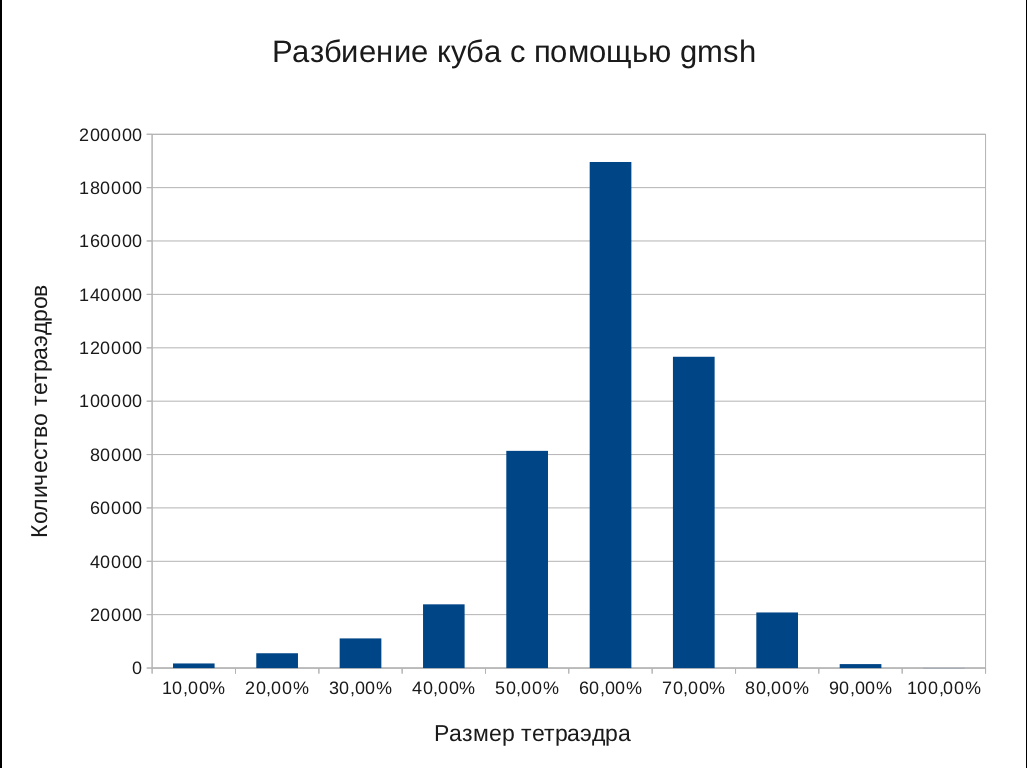
\includegraphics[width=\textwidth]{png/gmsh-stats.png}
\caption{Генератор gmsh.}
\end{subfigure}
\begin{subfigure}[b]{0.5\textwidth}
\centering
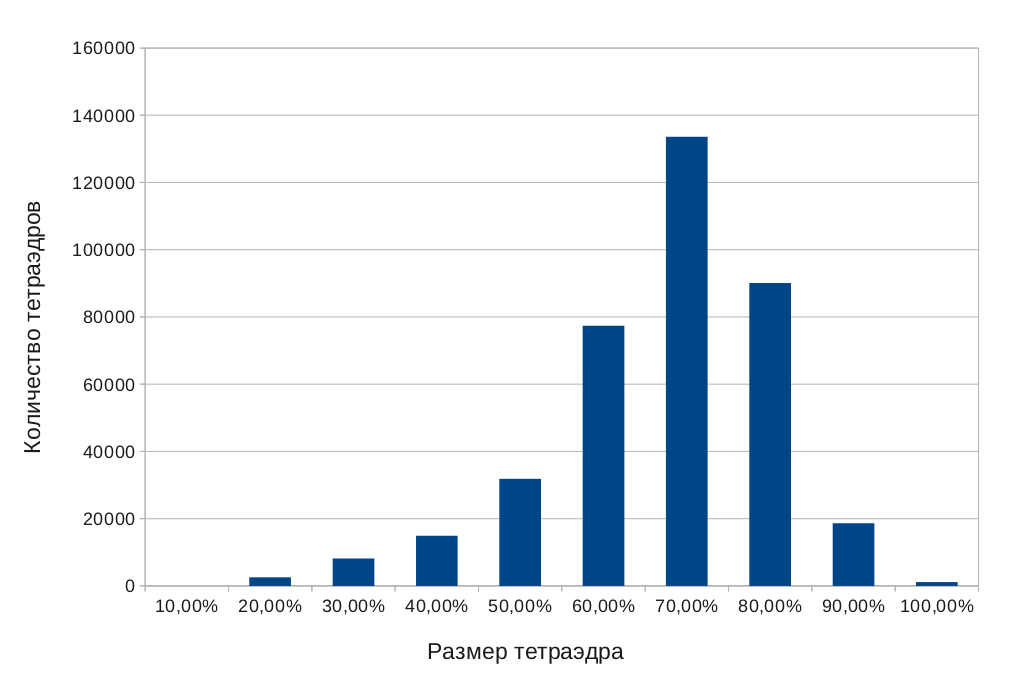
\includegraphics[width=\textwidth]{png/tetgen-stats.png}
\caption{Генератор tetgen.}
\end{subfigure}
\begin{subfigure}[b]{0.5\textwidth}
\centering
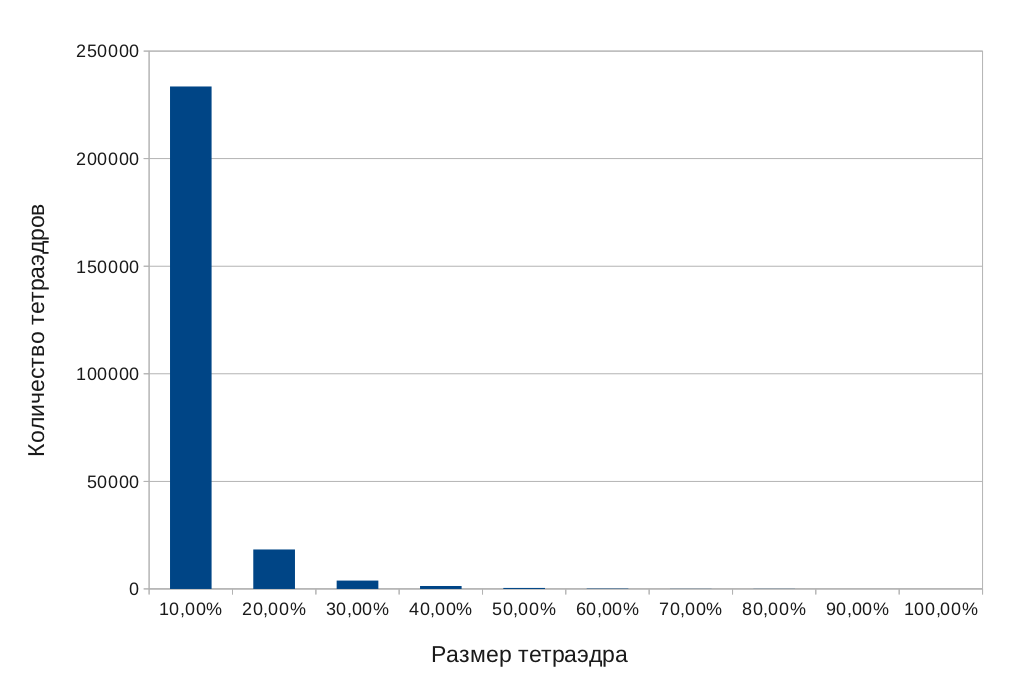
\includegraphics[width=\textwidth]{png/ani3d-stats.png}
\caption{Генератор Ani3D.}
\end{subfigure}
\begin{subfigure}[b]{0.5\textwidth}
\centering
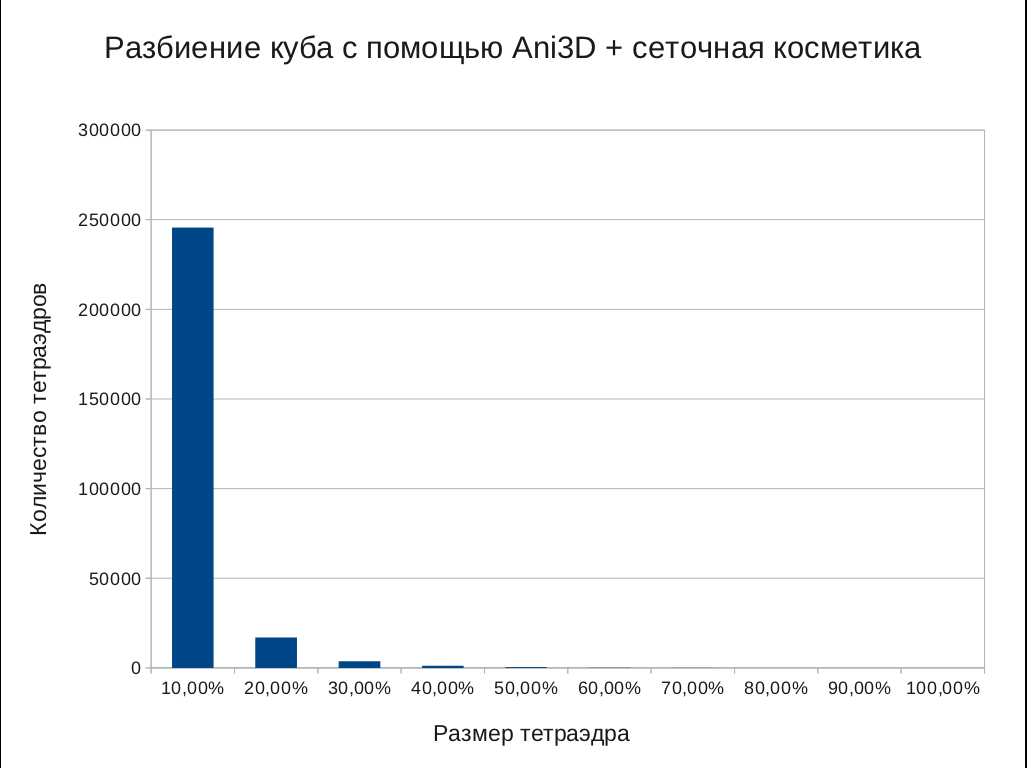
\includegraphics[width=\textwidth]{png/ani3d-improved-stats.png}
\caption{Генератор Ani3D с сеточной косметикой.}
\end{subfigure}
\caption{Сетка в кубе, созданная различными генераторами. Распределение тетраэдров по размеру.}
\label{pic:mesh_quality}
\end{figure}

\clearpage
\newpage

\subsubsection{Конструирование метода}

Рассмотрим одномерное уравнение переноса

\begin{equation}
\frac{\partial{u}}{\partial{t}} + \lambda \frac{\partial{u}}{\partial{x}} = 0, \lambda \ne const.
\end{equation}

Введем в области интегрирования разностную сетку и обозначим $u_m^n = u(t^n, x_m)$. Обратим внимание, что мы изначально предполагаем неравномерность сетки. Это соответствует как случаю с изначально сеткой низкого качества, так и случаю больших деформаций и вырождения сетки. Кроме того, мы рассматриваем случай разных значений $\lambda$ в разных точках расчетной области. Такая ситуация имеет место, если среда изначально неоднородная или если большие деформации вызвали значительное локальное изменение плотности в точке.

Особенностью предлагаемого метода является тот факт, что на данном этапе не будем выбирать фиксированный сеточный шаблон. Необходимые точки на предыдущем временном слое, по которым выполняется реконструкция значений на следующем шаге по времени, будут определяться в ходе вычислений отдельно для каждой рассчитываемой точки, исходя из локальных свойств решения в ней.

Предположим, что из тех или иных соображений был выбран шаг по времени $\tau$, такой что характеристика из точки $u_m^n$ не попадает в отрезок $(u_{m-1}^n; u_{m+1}^n)$.

В этом случае найдем тот отрезок $(u_{m-k-1}^n; u_{m-k}^n)$, в котором выпущенная характеристика пересекает временной слой $n$. Точку пересечения обозначим $x^*$. Также введем обозначения:
\begin{align}
x_{m-k} - x_{m-k-1} &= h_k,\nonumber\\
x_m - x^* = \lambda \tau &= l_0,\nonumber\\
x_m - x_{m-k} &= l_k.
\end{align}

Нормируя $l_k$ и $l_0$ на $h_k$ получаем:
\begin{align}
q_0 &= l_0 / h_k = \lambda \tau / h_k = \sigma,\nonumber\\
q_k &= l_k / h_k,
\end{align}
где $\sigma$ -- аналог классического числа Куранта для равномерной сетки.

Рассмотрим простейший случай линейной интерполяции значения в точке $u_*^n$ по точкам  $u_{m-k-1}^n$ и $u_{m-k}^n$. Получаем для значения на новом временном слое $u_m^{n+1}$ следующее выражение:
\begin{align}
\label{newmethod_1d_scheme}
u_m^{n+1} = u_*^n = (q_k + 1 - q_0) u_{m-k}^n + (q_0 - q_k) u_{m-k-1}^n.
\end{align}


\subsubsection{Исследование метода}

Чтобы найти порядок аппроксимации по времени и по пространству используем разложение $u_{m+\mu}^{n+\nu}$ в ряд Тейлора. Обозначим:
\begin{align}
q_0 - q_k &= \sigma_k,\nonumber\\
\frac{h_k}{l_0} &= \alpha,\nonumber\\
\frac{l_k}{l_0} &= \beta,
\end{align}
где очевидно $\alpha < 1, \beta < 1$.

Раскладывая \ref{newmethod_1d_scheme} в ряд Тейлора в окрестности $u = u_m^n$ до второго порядка малости получаем:
\begin{align}
u + u_\tau \tau + u_{\tau\tau} \frac{\tau^2}{2} &= (1 - \sigma_k) (u - l_k u_x + u_{xx} \frac{l_k^2}{2}) + \nonumber\\
	&+ \sigma_k (u - (l_k+h_k) u_x + u_{xx} \frac{(l_k+h_k)^2}{2}) \nonumber\\
u_\tau \tau + u_{\tau\tau} \frac{\tau^2}{2} &= (1 - \sigma_k) (- l_k u_x + u_{xx} \frac{l_k^2}{2}) + \nonumber\\
	&+ \sigma_k (- (l_k+h_k) u_x + u_{xx} \frac{(l_k+h_k)^2}{2}) \nonumber\\
u_\tau \tau + u_{\tau\tau} \frac{\tau^2}{2} &= - u_x ( (1 - \sigma_k) l_k + \sigma_k (l_k+h_k) ) + \nonumber\\
	&+\frac{u_{xx}}{2} ( (1 - \sigma_k) l_k^2 + \sigma_k (l_k+h_k)^2 ) \nonumber\\
u_\tau \tau + u_x  ( l_0 ) &= - u_{\tau\tau} \frac{\tau^2}{2} + \frac{u_{xx}}{2} ( l_k^2 + 2 \sigma_k l_k h_k + \sigma_k h_k^2 ) \nonumber\\
u_\tau \tau + u_x  \lambda \tau &= - u_{\tau\tau} \frac{\tau^2}{2} + \frac{u_{xx}}{2} ( l_k (l_k + \sigma_k h_k) + \sigma_k h_k (l_k + h_k) ) \nonumber\\
u_\tau \tau + u_x  \lambda \tau &= - u_{\tau\tau} \frac{\tau^2}{2} + \frac{u_{xx}}{2} ( l_k l_0  + \sigma_k h_k l_0 (\alpha + \beta) ) \nonumber\\
u_\tau + u_x  \lambda &= - u_{\tau\tau} \frac{\tau}{2} + \frac{u_{xx}}{2} \lambda ( l_k  + \sigma_k h_k (\alpha + \beta) ) \nonumber\\
u_\tau + u_x  \lambda &= O(\tau) + O (h)
\end{align}

Таким образом, схема имеет первый порядок по времени и по пространству. Этого следовало ожидать, так как используемая линейная интерполяция имеет первый порядок точности.

Для исследования устойчивости воспользуемся методом Фурье. Рассмотрим $u_m^n = v^n e^{im\phi}$. Подставив его в \ref{newmethod_1d_scheme} получим:
\begin{align}
v^{n+1} e^{im\phi} &= (q_k + 1 - q_0) v^{n} e^{i(m-k)\phi} + (q_0 - q_k) v^{n} e^{i(m-k-1)\phi} \nonumber\\
v^{n+1} e^{im\phi} &= v^{n} e^{im\phi} ((q_k + 1 - q_0) e^{-ik\phi} + (q_0 - q_k) e^{-i(k+1)\phi} \nonumber\\
u_m^{n+1} &= u_m^n ((q_k + 1 - q_0) e^{-ik\phi} + (q_0 - q_k) e^{-i(k+1)\phi}).
\end{align}

Таким образом, оператор перехода от слоя $n$ к слою $n+1$ имеет вид:
\begin{align}
\lambda = e^{-ik\phi} ( 1 + (q_k - q_0) (1 - e^{-i\phi}) ).
\end{align}

Необходимое условие устойчивости Неймана:
\begin{align}
|\lambda|^2 &\le 1 \nonumber\\
| 1 + (q_k - q_0) (1 - e^{-i\phi}) |^2 &\le 1 \nonumber\\
| 1 + (q_k - q_0) (1 - \cos(\phi)) + i(q_k - q_0)\sin(\phi) |^2 &\le 1 \nonumber\\
( 1 + (q_k - q_0) (1 - \cos(\phi)))^2 + ((q_k - q_0)\sin(\phi))^2 &\le 1 \nonumber\\
( 1 + q_k - q_0)^2 - 2 ( 1 + q_k - q_0)(q_k - q_0) \cos(\phi) + (q_k - q_0)^2 &\le 1 \nonumber\\
1 + 2 (q_k - q_0) + 2 (q_k - q_0)^2 - 2 ( 1 + q_k - q_0)(q_k - q_0) \cos(\phi) &\le 1 \nonumber\\
(q_k - q_0)^2 - (q_k - q_0) ( 1 + q_k - q_0 ) \cos(\phi) + (q_k - q_0) &\le 0 \nonumber\\
(q_k - q_0)(q_k - q_0 + 1)(1 - \cos(\phi)) &\le 0 \nonumber\\
(q_k - q_0)(q_k - q_0 + 1) &\le 0
\end{align}

Отсюда получаем
\begin{align}
-1 &\le q_k - q_0 \le 0,  \nonumber\\
q_k &\le q_0 \le q_k + 1.
\end{align}

Таким образом, схема устойчива при 
\begin{align}
k \le \sigma \le k+1.
\end{align}

Так как все коэффициенты схемы неотрицательны, то она также является монотонной в соответствии с критерием Фридрихса.

Полученное условие де-факто эквивалентно условию попадания характеристики в отрезок, по которому производится интерполяция. Если для реконструкции решения используется интерполяция более высоких порядков, то необходимый сеточный шаблон будет расширяться. Например, для интерполяции второго порядка необходимо использовать три точки на временном слое $n$. В этом случае можно выбрать любой из трехточечных шаблонов, включающих в себя $x^*$ -- $(u_{m-k-2}^n; u_{m-k}^n)$ или $(u_{m-k-1}^n; u_{m-k+1}^n)$. В общем случае, в соответствии с \cite{magomedov}, все схемы с порядком аппроксимации выше первого не будут монотонны.

\clearpage
\newpage

\subsubsection{Тестирование метода}

На рис. \ref{pic:scheme_1d_test} приведены результаты тестирования описанной схемы. Рассматривалась задача распада разрыва. Использовалась равномерная сетка по пространству. Приведены графики для расчетов с $\lambda \tau / h = 1.0$ (классический шаблон "уголок" с курантовским шагом) и $\lambda \tau / h = 1.5$ (описанная выше схема).

\begin{figure}[htp]
\begin{subfigure}[b]{0.5\textwidth}
\centering
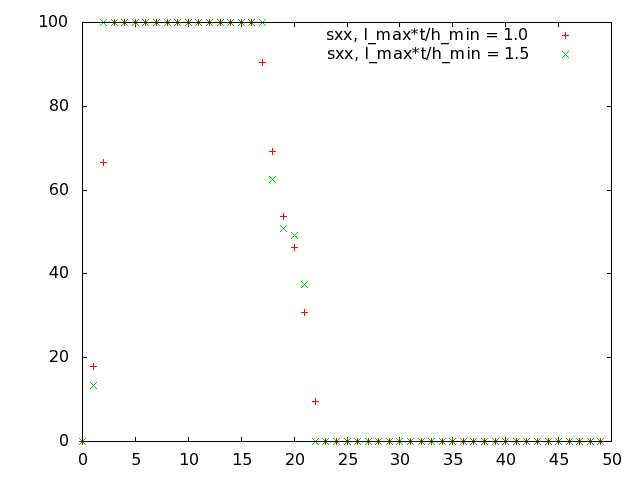
\includegraphics[width=0.8\textwidth]{png/big-sigma-test-results-1d/snap-1.png}
\caption{1-ый шаг по времени.}
\end{subfigure}
\begin{subfigure}[b]{0.5\textwidth}
\centering
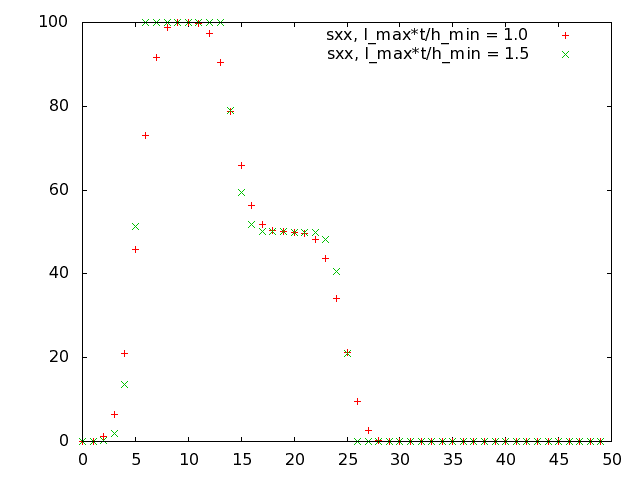
\includegraphics[width=0.8\textwidth]{png/big-sigma-test-results-1d/snap-3.png}
\caption{3-ий шаг по времени.}
\end{subfigure}
\begin{subfigure}[b]{0.5\textwidth}
\centering
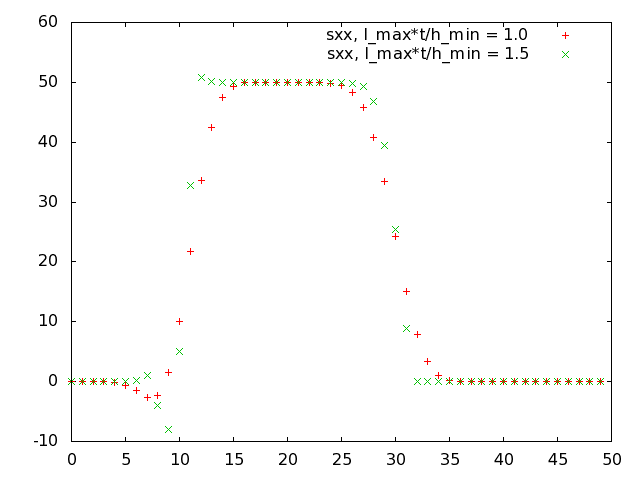
\includegraphics[width=0.8\textwidth]{png/big-sigma-test-results-1d/snap-6.png}
\caption{6-ой шаг по времени.}
\end{subfigure}
\begin{subfigure}[b]{0.5\textwidth}
\centering
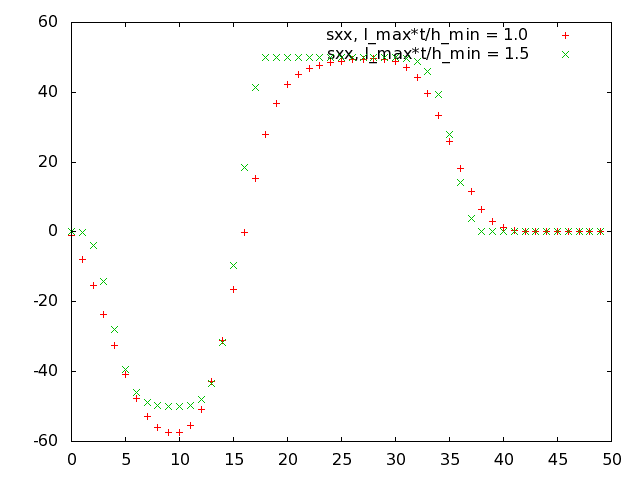
\includegraphics[width=0.8\textwidth]{png/big-sigma-test-results-1d/snap-9.png}
\caption{9-ый шаг по времени.}
\end{subfigure}
\begin{subfigure}[b]{0.5\textwidth}
\centering
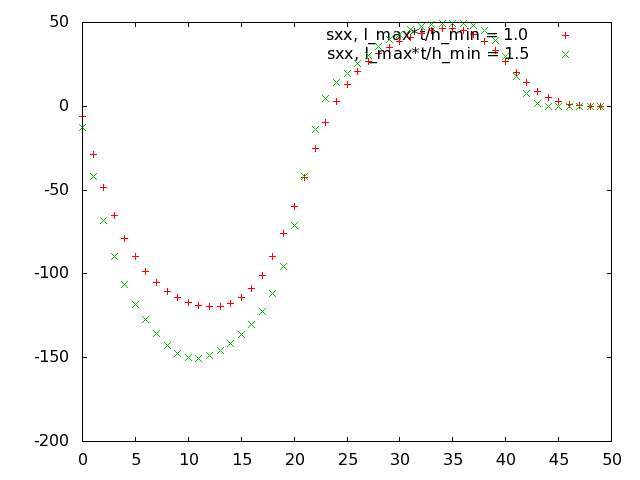
\includegraphics[width=0.8\textwidth]{png/big-sigma-test-results-1d/snap-12.png}
\caption{12-ый шаг по времени.}
\end{subfigure}
\begin{subfigure}[b]{0.5\textwidth}
\centering
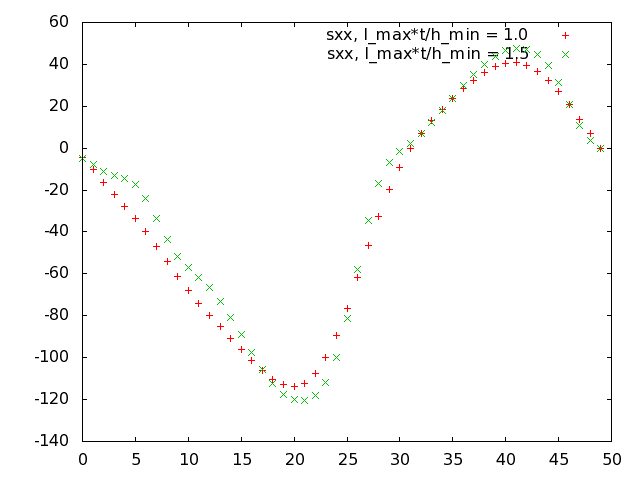
\includegraphics[width=0.8\textwidth]{png/big-sigma-test-results-1d/snap-15.png}
\caption{15-ый шаг по времени.}
\end{subfigure}
\caption{Тестирование одномерной схемы с шагом $\lambda \tau / h = 1.5$.}
\label{pic:scheme_1d_test}
\end{figure}


\subsubsection{Работа на неструктурированной сетке из тетраэдров}

Для решения многомерной задачи с большим шагом по времени ($\lambda \tau / h > 1$) используется описанный выше метод для одномерной задачи и схема расщепления по пространственным переменным. Схема расщепления конструируется ровно так же, как для случая с классическим курантовским шагом. Используется случайный выбор базиса для симметризации решения без излишнего увеличения вычислительной сложности задачи.

Расчёт внутренних, граничных и контактных узлов при таком подходе не вызывает проблем -- для каждой одномерной схемы находятся элементы сетки на прошлом временном слое, в которые попали характеристики. Для внутренних узлов все 9 характеристик оказываются внутри расчётной области, из соответствующих точек переносятся инварианты Римана и по ним восстанавливется решение на новом временном слое. Для граничных узлов 6 характеристик попадают внутрь области, а 3 уравнения, соответствующие выводящим характеристикам, заменяются на граничные условия. Для узлов на контактной границе решается система из 18 уравнений, записанных в двух соприкасающихся узлах, -- постановка контактных условий и расчёт полностью аналогичны описанному выше для случая с классическим курантовским шагом.

Отдельного подхода при расчёте с шагом по времени $\tau > h / \lambda$ требуют приграничные узлы. Они являются внутренними для расчётной области и должны рассчитываться по схеме для внутренних узлов -- по 9 значениям инвариантов Римана, перенесённым с прошлого временного слоя, и без привлечения граничных или контактных условий. Однако, в силу большого шага по времени, для узлов, расположенных достаточно близко к границе области, могут возникать характеристики, которые выходят за границы области на предыдущем временном слое.

В этом случае требуется переносить значения инвариантов Римана из виртуальных узлов, расположенных между временными слоями $n$ и $n+1$. Иллюстрация такой ситуации приведена на рис. \ref{pic:near_border_node}.

\begin{figure}[htp]
\centering
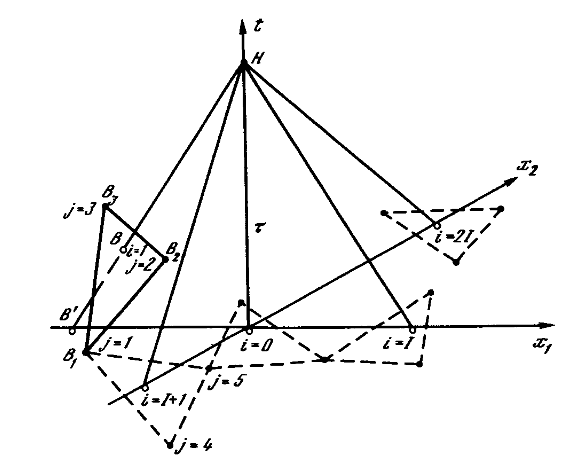
\includegraphics[width=0.6\textwidth]{png/characteristics-2d-triangles-semi-border.png}
\caption{Расчет узла, близкого к границе.}
\label{pic:near_border_node}
\end{figure}

Для одной из характеристик точка пересечения с предыдущим временным слоем оказалась за границей области интегрирования (точка $B'$). В этом случае значение переносится из точки $B$, значение в которой интерполируется по точкам $B_1, B_2, B_3$, причем точки $B_1$ и $B_2$ находятся на старом временном слое, а точка $B_3$ -- на новом. Очевидно, что при таком подходе при реализации метода требуется предусмотреть в алгоритме расчёта последовательность вычисления значений на новом временном слое -- сначала вычисляются значения в граничных узлах, после чего начинается расчёт внутренних точек.


\subsubsection{Движение сетки при больших деформациях}

Одной из традиционных проблем при расчёте задач с конечными деформациями является вырождение шага по времени из-за искажения ячеек расчётной сетки. Традиционный подход к решению этой проблемы -- перестройка сетки при появлении деформаций, переинтерполяция на новую сетку и продолжение счёта на новой сетке.

Предложенный метод расчёта с $\tau > h / \lambda$ позволяет предложить альтернативный подход к решению данной проблемы -- при искажении ячеек расчётной сетки просто продолжается счёт с прежним шагом по времени, для искажённых ячеек сетки соотношение $\lambda \tau / h$ может принимать достаточно большие значения, что обрабатывается внутренней логикой метода.

Все выполненные в рамках данной работы расчёты используют именно такой подход.

